\section{Pie Chart \cite{data/online/matplotlib.pyplot.pie}} \label{Visualizing Data/Pie Chart}


\begin{table}[H]
\begin{minipage}[t]{0.35\linewidth}
\begin{figure}[H]
    \centering
    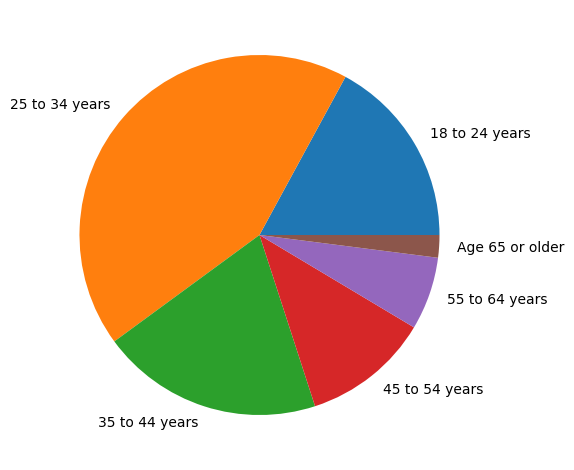
\includegraphics[width=0.9\linewidth, height=10cm, keepaspectratio]{images/data/__visualizations__/plt-pie-age-face-data.png}
    \caption{Pie chart (py-plt) output (face\_data.csv)}
\end{figure}
\end{minipage}
\hspace{0.2cm}
\vrule width 1pt
\hspace{0.5cm}
\begin{minipage}[t]{0.57\linewidth}
\begin{lstlisting}[
    language=Python,
    caption=Pie Chart: py-plt: face\_data.csv
]
vals = df[df["age"] != " "].copy()

labels, counts = np.unique(
    vals['age'],
    return_counts=True
)

plt.pie(counts, labels=labels)

plt.tight_layout()
plt.show()
\end{lstlisting}
\end{minipage}
\end{table}

